\documentclass[a4paper,11pt]{article}
\usepackage[utf8]{inputenc}
\usepackage{algorithmic}
\usepackage{algorithm}
\usepackage{pst-plot}
\usepackage{graphicx}
\usepackage{endnotes}
\usepackage{graphics}
\usepackage{floatflt}
\usepackage{wrapfig}
\usepackage{amsfonts}
\usepackage{amsmath}
\usepackage{verbatim}
\usepackage{hyperref}
\usepackage{multirow}
\usepackage{pdflscape}
 \usepackage{enumitem}

\usepackage{hyperref}
\hypersetup{pdfborder={0 0 0 0}}

\pdfpagewidth 210mm
\pdfpageheight 297mm 
\setlength\topmargin{0mm}
\setlength\headheight{0mm}
\setlength\headsep{0mm}
\setlength\textheight{250mm}	
\setlength\textwidth{159.2mm}
\setlength\oddsidemargin{0mm}
\setlength\evensidemargin{0mm}
\setlength\parindent{7mm}
\setlength\parskip{0mm}

\newenvironment{exercise}[3]{\paragraph{Exercise #1: #2 (#3pt)}\ \\}{
\medskip}
\newcommand{\question}[2]{\setlength\parindent{0mm}\ \\$\mathbf{Q_#1:}$ #2\ \\}

\author{\large{Ardi Tampuu, Ilya Kuzovkin, Raul Vicente}}
\title{\huge{Introduction to Computational Neuroscience}\\\LARGE{Practice Session on Machine Learning}}

\begin{document}
\maketitle

\textbf{HINT: } There is a file called \texttt{sample.m} in the code folder. It does not provide sample code, but it summarizes the steps to follow. It works for both exercises. Some helpful functions are in \texttt{code/helpers/} folder.

\vspace{0.8cm}
%
% Intro
%
The main purpose of the fields of \emph{neural encoding} and \emph{neural decoding} is to learn the relation between a stimulus and the neural response elicited by this stimulus. When studying \emph{encoding} we want to predict how the brain would respond given a certain stimulus - we estimate the probability $p(brain response | stimulus)$. In neural decoding we do the inverse - we read the brain activity using imaging techniques and ask the question "which stimulus caused this activity?" - we look for $p(stimulus | brain response)$. 

In a decoding paradigm we we present the test subjects with different stimuli while at the same time recording responses on their brains. The task is to create a \emph{model}, which takes any piece of the recorded brain data as an input and \emph{predicts} which stimulus was responsible for producing this piece of data.

In the last practice session we kind of \emph{manually} created one such model: by looking at the firings of 72 neurons we might pretty accurately guess the orientation of the bar on the screen. We would be able to predict which stimulus was shown, given the neural responses. Nevertheless, very often the data can be too massive or too complex to find such direct relation between activity and stimulus by simple observation. That's where \emph{machine learning} comes to our aid.

The main goal of machine learning can be summarized as providing an automatic way of finding the dependencies between a set of features (neural data) and the corresponding labels (the stimuli).\\


%
% ML introduction
%
Before we continue let us go through vocabulary:
\begin{itemize}
\itemsep 0em
	\item \textbf{A dataset} is a structure which contains all the data we have.
	\item A dataset consist of \textbf{instances}, often also referred to as data points.
	\item In case of classification, instances consist of \textbf{features} and a \textbf{class label}.
	\item Features are parameters, which describe our data. For example the average spiking rate of a neuron might be a feature, the power of EEG in a certain frequency band might be a feature, etc. Each instance has its own values for each of the features.
	\item All feature values of an instance put together form a \textbf{feature vector}.
	\item Feature vector is a representation of the instance in the \textbf{feature space}.
	\item Each instance belongs to a certain \textbf{class} - the name/ID number of stimulus that caused the features. 
	\item The goal of a machine learning algorithm is to create a \textbf{model}, which can guess the class (\textbf{classify}) of the instance given only its feature vector. A good model should be able to do this also on previously unseen feature vectors (generalize).
	\item The model is created from examples. Those are instances for which the class is known. A set of such examples is called \textbf{training set}, because we train our model on it.
	\item \textbf{Test set} is another set of instances, for which we also know the true class, but we do not share this knowledge with the model. Instead we ask the model to guess the class of each instance.
	\item We can then see how many instances from the test set model has identified correctly and the rate $$\displaystyle\frac{\text{Number of correctly classified instances}}{\text{Total number of instances}}$$ is called \textbf{accuracy}\footnote{Accuracy is a naive way to measure performance of the model. Read about \emph{precision} and \emph{recall} here \url{http://en.wikipedia.org/wiki/Precision_and_recall}} and it is used to evaluate model's performance.
\end{itemize}




\begin{exercise}{1.1}{Where is the rat?}{2}
In this task we will try to predict in which part of space a rat is located based on its neural activity. When collecting the data some electrodes were inserted to the rat's hippocampus where neurons responsible for navigation are located. At the same time the location of the rat was tracked by a camera. I have preprocessed the data so that:
\begin{enumerate}
\item \textbf{features} are spike counts in different neurons during a 500ms interval
\item \textbf{class} corresponds to which of the 16 areas the rat was located during these 500ms
\item your goal is to create a model that predicts the area based on the neural activity.
\end{enumerate}

\begin{wrapfigure}{r}{0.5\textwidth}
	\centering
	\vspace{-5pt}
	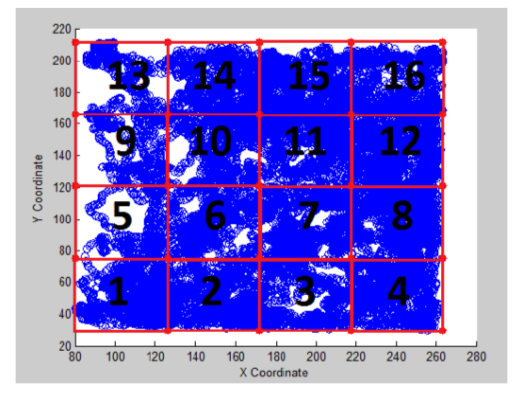
\includegraphics[width=0.45\textwidth]{rat.png}
	\caption{Find in which zone the rat is!}
	\label{fig:rat}
	
\end{wrapfigure}

In the \emph{data} folder you find a file called \emph{$rat\_data.mat$}, which contains the features(spike counts from 71 neurons), the classes (which sector) and the coordinates (not used in this exercise). The same information is also available in plain text format in .txt files.

Matlab and especially Octave is not the perfect tool for machine learning, so if you prefer other languages to solve this exercise, please do so. I especially recommend scikit-learn package in Python. Nevertheless, as the default language of this class is Matlab, I will provide instructions and helpful code in Matlab and not other languages.

Before the task you might need to install some packages such as (nan, statistics, io ...). To do that in Octave command window, hopefully the following command works:\\
\begin{center}
pkg install -auto -forge $PACKAGE\_NAME$
\end{center} 


\textbf{Your task is to:}
\begin{enumerate}
\item Read in the data and make sure you understand what is what
\item Randomly divide the instances into training and test sets, so that 80 percent of the data is in training set. \textbf{HINT:} there is a function in \texttt{code/helpers} folder that splits the data given features, labels and proportion
\item read how to use the \texttt{classify}\footnote{http://se.mathworks.com/help/stats/classify.html} function, so you would place training and test features and class labels in correct positions. Use "LDA" (linear discriminant analysis) as the type of classifier.\\
\textbf{For people not using Matlab:} whatever software you use, you need to perform Linear Discriminant Analysis.
\item Learn a model using the examples in the training set. Predict the locations for instances in test set and compare them with the true locations.
\item How much is the overall accuracy in the test set? How much is the precision for each class separately (return 16 values)?\\
\begin{center}
$precision\_of\_class\_i=\frac{points\ in\ zone\ i\ correctly\ classified\ as\ i}{total\ number\ of\ points\ classified\ as\ in\ zone\ i}$
\end{center}
\textbf{HINT:} class accuracies can be calculated by dividing the diagonal values of confusion matrix with the column sums 
\item use the \emph{$plot\_confmatrix(groundtruth, predictions)$} from \texttt{helpers} folder to draw a \textbf{confusion matrix}. What additional information (beyond class accuracies) does this matrix provide?
\item \textbf{For people not using Matlab:} you need to produce a confusion matrix, but it does not need to be a nice colourful drawing. It can also be just a readable (!!) printout of the matrix.
\end{enumerate} 
\end{exercise}

%
% Questions
%
\begin{exercise}{1.2}{A few questions to keep in mind}{1}
(answer in more than 1 phrase)
\question{1}{Why do you need to separate training and test datasets, that is why can't you evaluate your model on the training set? What does it mean if you accuracies on training set and test set are very different?}
\question{2}{If our model would just predict class labels completely randomly, what would be the average prediction accuracy?}
\question{3}{If our model would always predict the class label that is the most common label in our dataset, what would the average accuracy be?}
\end{exercise}

\pagebreak
%
% fMRI
%
\begin{exercise}{2}{Which picture was shown?}{2}
\begin{wrapfigure}{r}{0.4\textwidth}
	\centering
	\vspace{-45pt}
	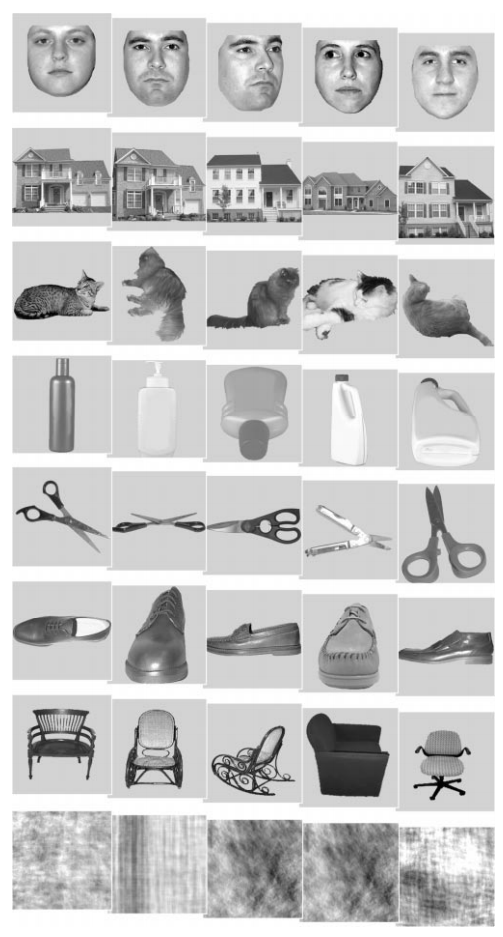
\includegraphics[width=0.35\textwidth]{stimuli.png}
	\caption{Examples of stimuli.}
	\label{fig:stimuli}
	\vspace{-20pt}
\end{wrapfigure}
In this exercise we will work with fMRI dataset\footnote{\url{https://openfmri.org/dataset/ds000105}} by Haxby et al.\footnote{\url{http://www.cs.pomona.edu/~syang/arch/visual_decoding/haxby_2001pdf.pdf}}. As you may recall, fMRI measures the blood oxygen level in the brain with high spatial precision. The data was recorded while test subject was presented with images from 9 categories: (1) house,  (2) scrambled, (3) cat, (4) shoe, (5), bottle, (6) scissors, (7) chair, (8) face, (9) something else. You can see them (except for the ``something else" category) on the Figure \ref{fig:stimuli}. The data we have is already preprocessed, so instead of $\approx$25000 voxels in the whole brain we only use 577 voxels from relevant brain areas. In machine learning terminology this means that each instance has 577 features and belongs to one of the 9 classes. You will find the feature data in \texttt{data/voxels.mat} and class information \texttt{data/labels.mat}. First one is 1492$\times$577 matrix (1492 instances 577 features each) and the second one is a vector of length 1492 (each instance has a class).

The question we want to answer is: \emph{Is is possible to decode from the fMRI signal the image the test subject was looking at?}. Your task will once again be to use Matlab \texttt{classify}\footnote{http://se.mathworks.com/help/stats/classify.html} function to build a predictive model.\\

Perform the following steps and report the results:
\begin{enumerate}
	\item Load the data. (Look at it. Always look at the data)
	\item Split data into training and test set. We want to have enough instances of each class in the test set to calculate meaningful statistics, so this time take only 70 $\%$ instances for training set).
	\item Classify using "LDA" as function type like before
	\item Use training set to train a model. With the model predict the classes of the test set.
	\item For each class calculate the precision on test set. Which class of images was the easiest to predict based on fMRI data? Which one was the hardest?
	\item \textbf{For people not using Matlab:} Train a LDA (Linear Discriminant Analysis) model on this data, using 80/20 train/test split. Answer the questions.
\end{enumerate}
\end{exercise}

------------------------------------  End of obligatory exercises  --------------------------
%
% Precision and Recall
%
\begin{exercise}{3*}{Precision, Recall, F1-score}{Bonus 1}
Sometimes accuracy can fail us if we are dealing with unbalanced datasets. If we classify images of cats and dogs and in out test set we have 90 $\%$ of cats, it is possible to achieve accuracy of 0.9 by simply always answering "cat". One possible countermeasure is to look not at the accuracy of the model, but at its \emph{precision} and \emph{recall}. 

Imagine you have 2 classes: "cat" and "dog". Precision is calculated for each class separately and shows how many of the instances the model has identified as cats are really cats. For example if out of 10 instances classified as "cats" two turn out to be "dogs" we say that precision is 0.8.

Recall is also calculated separately for each class. It shows how many of all cats present in the test set your model correctly identified as such. For example if there were 100 cats and 100 dogs and our model correctly classified only 78 cats (other 22 it guessed as dogs)  we say that its recall is 0.78.

F1 score is a convenient metric to write precision and recall as one number:
$$F1 = 2 \cdot \frac{\text{precision} \cdot \text{recall}}{\text{precision} + \text{recall}}$$
Your task is to calculate precision, recall and f1-score for each of 9 classes.
\end{exercise}

\ \\
\ \\
\ \\
\ \\
\ \\
Please submit a \texttt{pdf} report with answers to the questions and comments about your solutions. Include figures, explanations. Include the code within the pdf or as a separate file (zip them together). Upload it on the practice session page on the course website. Please mark how long it took to complete this set of exercises.
\end{document}










